\documentclass{csse4400}

\usepackage{CJKutf8}
\usepackage{languages}

\title{Scalable Text-to-Speech}
\author{Brae Webb}
\date{Semester 1, 2022}

\begin{document}
\maketitle

\section*{Summary}
In this assignment, you will demonstrate your ability to \textsl{design},
\textsl{implement}, and \textsl{deploy} a web application that can process a high load,
i.e. a scalable application.
You will be asked to deploy a tool that accepts text input and generates synthesized speech output.
Specially you need to support:
\begin{itemize}
    \item Uploading and generating speech for text input of varying sizes.
    \item Access via a specified REST API for use by front-end interfaces.
    \item Remaining responsive to the user while generating speech.
\end{itemize}

Your service will be deployed to AWS and will undergo automated correctness and load-testing to ensure it meets the required scalability.

\section{Introduction}
Text-to-speech software supports accessibility,
enables smart-home devices,
and even breaks down language barriers.
Unfortunately, text-to-speech is computationally intensive.
While the technology has made great advances over the past few decades,
many open-source implementations are still inefficient.

\paragraph{Task}
For this assignment,
the University of Queensland is looking to convert all course content into speech.
This will support visually impaired students in their studies.
All course content from slack messages and blackboard announcements to textbooks must be converted to speech.
You will be responsible for designing and implementing a service to generate synthesized speech for use across the entire university.

\paragraph{Requirements}
As you might imagine,
blackboard announcements occur frequently and should be translated in almost real time.
While textbooks are set ahead of semester and may take several days to process.
The university will experience peaks of usage.
At the start of semester,
instructors set many textbooks which need to be processed.
The university will also experience usage lows over the summer holiday period when few translations will be required.
The university is not willing to pay for the resources required during usage peaks all year round.
Your implementation must be able to scale dynamically based on the current amount of jobs to be processed.

% \section{Features}


\section{Interface}
Your service will be utilised by almost every system in the university.
Every university service must support text-to-speech on the first Monday of semester two.
An interface specification has already been developed and distributed to existing service owners,
who are working hard to deliver support for their services.

You must implement this interface exactly as described.
The interface specification is available to all service owners online:
\url{https://csse6400.uqcloud.net/assessment/chatterbox}

\section{Implementation}
To ensure that your service is able to faithfully generate voice clips that our tests will expect,
there are some restrictions on how your service can be implemented.

Your service must utilise the chatterbox command line tool provided for this assignment.
This tool is available on pypi and may be installed using pip: \url{https://pypi.org/project/uq-chatterbox/}

\section{Submission}
Your solution must committed to the GitHub repository specified in Section \ref{sec:github}.
Committing to this repository will be disabled after \textbf{16:00 (AEST) on 6 May 2022} and the contents of the repository at this time will be taken as your submission.
The repository \textbf{must} contain everything required to successfully deploy your application.
You must include all of the following in the repository:
\begin{itemize}
  \item Your implementation of the service API, including the source code and a mechanism to build the service.%
  \footnote{If you are using external libraries, ensure that you pin the version to avoid external changes breaking your application.}
  \item Terraform code that can provision your service from a fresh AWS learner lab environment.
\end{itemize}

When deploying your application to mark,
we will follow reproducible steps, outlined below.
You may re-create the process yourself.

\begin{enumerate}
  \item Your Git repository will be checked out locally.
  \item AWS credentials will be copied into your repository in the top-level directory,
  in a file called \texttt{credentials}.
  \item The script \texttt{deploy.sh} in the top-level of the repository will be run.
  \item The \texttt{deploy.sh} script \textbf{must} create a file named \texttt{api.txt} which contains the URL where your API is deployed to.
  \item We will run automated functionality and load-testing on the URL provided in the \texttt{api.txt} file.
\end{enumerate}

\subsection{GitHub Repository}\label{sec:github}
You will be provisioned with a private repo on GitHub for this assignment, via GitHub Classroom.
You must click on the link below and associate your GitHub username with your UQ student id in the Classroom.

\url{https://classroom.github.com/a/tGJ8UEBh}\\
Associating your GitHub username with another student's id,
or getting someone else to associate their GitHub username with your student id, is \link{academic misconduct}
{https://my.uq.edu.au/information-and-services/manage-my-program/student-integrity-and-conduct/academic-integrity-and-student-conduct}.

If for some reason you have accidently associated your GitHub username with the wrong student id,
contact the course coordinator as soon as possible.

\subsection{Tips}

\paragraph{Outputting an API URL}
Your Terraform code should produce a URL from where your API can be accessed.
A requirement is that this URL is stored in the file \texttt{api.txt}.
We recommend that you use the \texttt{local\_file} resource to accomplish this.

\begin{code}[language=terraform]{}
resource "local_file" "url" {
    content  = # some resource output here
    filename = "./api.txt"
}
\end{code}

\paragraph{Terraform apply in deploy script}
Your \texttt{deploy.sh} script must deploy without user interaction.
You can run Terraform apply without prompting for configuration using the command:
\bash{terraform apply -auto-approve}

\paragraph{If something goes wrong}
Ideally, your infrastructure will be deployed successfully but this could go wrong for any number of unforeseen reasons.
If something does go wrong during deployment,
teaching staff will refer to your \texttt{README.md} file to attempt to resolve the issue where possible.
Please ensure that your \texttt{README.md} documentation is of high quality to allow yourself the best chance for recovery.

\paragraph{Terraform plan/apply hanging}
If your \texttt{terraform plan} or \texttt{terraform apply} command hangs without any output,
check your AWS credentials.
Using credentials of expired learner lab sessions will cause hanging.

\paragraph{Fresh AWS learner lab}
Your AWS learner lab can be reset using the reset button in the learner lab toolbar.
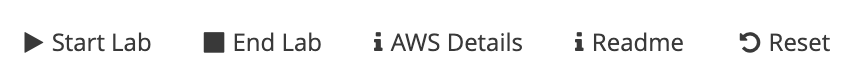
\includegraphics[width=\textwidth]{images/reset-button.png}
To ensure that you are not accidentally depending on anything specific to your learner lab environment,
we recommend that you reset your lab prior to final submission.
Note that resetting the lab can take a considerable amount of time,
in the order of hours, you should do this at least 4 to 6 hours before the submission deadline.
Please do not wait to the last minute.

\paragraph{Deploying with Docker}
In this course,
you have been shown how to use Docker containers to deploy EC2 instances \cite{prac-week5}.
You may find it a pragmatic way to deploy your application in this assignment.
If you intend to deploy using Docker containers,
we recommend that you create a GitHub actions workflow
to build and publish your container to the GitHub container registry.
An example of this can be seen in the \link{todo-app}{https://github.com/CSSE6400/todo-app/blob/main/.github/workflows/backend.yml}.
Containers can then be deployed from a ghcr URL, e.g. \url{ghcr.io/csse6400/todo-app}.

Containers deployed to the container registry will need to be \textbf{private}.
You will need to authenticate when pulling your container.
The current best approach is:

\begin{enumerate}
  \item Create a \link{Personal Access Token (PAT)}{https://github.com/settings/tokens/new} with \texttt{read:packages} permissions.
  \item Create a Terraform variable \texttt{github\_pat}.
\begin{code}[language=terraform]{}
variable "github_pat" {
    description = "A personal access token with read:packages permissions"
    type        = string
}
\end{code}
  \item Configure your EC2 provisioning script to login to docker with these credentials, e.g.
  \bash{echo \$\{GH\_PAT\} | docker login ghcr.io -u <username> --password-stdin}
  \item When running \texttt{terraform apply} ensure that the PAT is set as the environment variable,\\
  \texttt{TF\_VAR\_github\_pat}
  \bash{export TF_VAR_github_pat=<token>}
\end{enumerate}

When we run your \texttt{deploy.sh} script,
our environment will contain a \texttt{TF\_VAR\_github\_pat} with access to pull from your container registry.


\paragraph{Unique S3 buckets}
You may find it helpful to use S3 buckets for this assignment.
It is important to be aware that the name of an S3 bucket has to be \textsl{globally} unique.
To avoid any deployment conflicts,
we recommend that you use the \texttt{random\_string} Terraform resource.
This allows you to generate a random string which can be appended to the S3 bucket name.

\begin{code}[language=terraform]{}
resource "random_string" "bucket-name" {
    length    = 16
    special   = false
    upper     = false
}

resource "aws_s3_bucket" "bucket" {
    bucket = "my-bucket-${random_string.bucket-name.result}"
}
\end{code}

\paragraph{S3 pre-signed URLs}
If you are using AWS S3 to store audio recordings,
ensure that you consider the security aspects of storing these recordings.
You do not want to make your S3 bucket publicly accessible.
A good middle-ground is to use \link{pre-signed URLs}{https://docs.aws.amazon.com/AmazonS3/latest/userguide/ShareObjectPreSignedURL.html} which allow you to generate temporary URLs that have read access to an object in an S3 bucket, e.g.

\begin{code}[language=python]{}
import boto3
url = boto3.client('s3').generate_presigned_url(
  ClientMethod='get_object', 
  Params={'Bucket': BUCKET_NAME, 'Key': OBJECT_KEY},
  ExpiresIn=3600
)
\end{code}


\subsection{Fine Print}
You can reproduce our process for deploying your application using our \link{Docker image}{https://ghcr.io/CSSE6400/csse6400-cloud-testing}:
\codefile[language=docker]{Dockerfile}{deployment/Dockerfile}

\noindent
Our steps for deploying your infrastructure using this container are as follows.
\texttt{\$REPO} is the name of your repository,
\texttt{\$CREDENTIALS} is the path where we will store our AWS credentials,
and \texttt{\$GH\_PAT} is a personal access token with package read permissions:
\begin{code}[language=shell]{}
$ git clone git@github.com:CSSE6400/$REPO
$ cp $CREDENTIALS $REPO
$ docker run -v /var/run/docker.sock:/var/run/docker.sock -v $(pwd)/$REPO:/workspace --env TF_VAR_github_path=$GH_PAT csse6400-cloud-testing
$ cat $REPO/api.txt # this will be used for load-testing
\end{code}

\noindent
Note that the Docker socket of the host has been mounted,
this enables running \texttt{docker} in the container.
This has been tested on MacOSX and Linux but might require WSL2 on Windows.


\section{Criteria}
Your assignment submission will be assessed on its ability to support the specified use cases.
Testing is divided into functionality testing and quality testing.
Functionality testing is to ensure that your backend software and API meet the MVP requirements by satisfying the API specification without excessive load.
Quality testing is based upon several likely use case scenarios.
The scenarios create different scaling requirements.

Partial marks are available for both types of tests,
i.e. if some functionality is implemented you can receive marks for that functionality,
or if your service can handle 80\% of the load during quality testing you will receive marks for that.

\subsection{Functionality}
You will be awarded some credit for correct implementation of the API specification without being able to cope with excessive load.
A suite of automated API tests will assess the correctness of the implementation, via a sequence of API calls.
Some tests from this suite will be made available before the assignment due date.

\subsection{Quality Scenarios}\label{sec:scenarios}

\paragraph{Semester break}
Your application will see decreased usage during the semester break.
Minimal students and staff may periodically query pre-generated speech when revising content.
During this period we might see traffic of not more than 20 parallel users,
querying read-only endpoints.

% \begin{code}[language=javascript]{}
% stages: [
%   { duration: '1m', target: 10 },
%   { duration: '1m', target: 20 },
%   { duration: '1m', target: 0 },
% ]
% endpoints: [
%   get("/health"),
%   get("/text"),
%   get("/text/{id}")
% ]
% \end{code}

\paragraph{Exam revision}
During the 20 minutes prior to an exam of a larger course, such as CSSE1001,
you might expect the entire cohort, all one thousand users,
revising the content.
Revising the content will consist primarily of read-only requests.

\paragraph{Monday of exam block}
Courses with large enrollments tend to have their exam scheduled at the start of exam block.
This enables course staff the most possible time to mark these exam papers.
At 8am on Monday of exam block,
the 4 largest cohorts will begin using your service for revision.

In addition, teaching staff for exams later in the week have begun uploading revision material.
We might expect about 30 staff members to upload their one page course summaries,
about 3,500 characters each.

\paragraph{Teaching cancelled}
Queensland has seen `unprecedented' rainfall causing the university to flood.
The university admin have made the call to cancel teaching for the week.
Coordinators are responsible for disseminating this information to their students.
All 1,957 courses must send announcements averaging 100 characters (many exact copies of the suggested announcement),
to relay this information.

\paragraph{Reading list due date}
The library has a deadline for course coordinators to submit their course reading lists.
In this completely fictional example,
we can imagine that coordinators have left uploading their reading list until the last minute.
Suddenly your system receives a large amount of requests to generate the spoken version of textbooks (we will vastly under-estimate that textbooks are round 7,000 characters).
About 100 coordinators submit their reading list at the last minute.

\paragraph{In-semester Monday morning}
Each semester there are a small number of new courses running for the first time.
These courses, in an attempt to keep up with the passage of time,
upload the course material for the week on a Monday morning.
About 20 courses uploading 2,500 characters of material.
At the same time, many coordinators like to send our announcements on Monday mornings summarizing the weeks content.
These announcements are typically around 80 characters long and sent out by 75 or so coordinators.

\subsection{Marking}
Functionality accounts for 50\% of the marks for the assignment.
This is split as 30\% for correct implementation of the provided API,
and 20\% for correct implementation of the backend processing.
The simple queries in the API are worth much less of the mark compared to the API operations that require dealing with persistent data.
Note that the API marks are for \emph{implementing} the API, \emph{separate} to the backend functionality.
This means that an API operation that behaves correctly based on the specification will achieve full marks,
even if the backend processing is not working correctly.

Backend processing is the synchronous and asynchronous conversion of text to speech.
Synchronous processing is worth 12\% and asynchronous processing is worth 8\%.
All functionality marks are based solely on correct implementation of the functionality, as assessed by the automated functionality tests.

Scaling your application to deliver the quality scenarios accounts for the other 50\% of the marks.
The scenarios described in section \ref{sec:scenarios} provide guidance as to the type of scalability issues your system is expected to handle.
They are not literal descriptions of the exact loads that will be used.
Tests related to scenarios that involve more complex behaviour will have higher weight than other tests.

Scaling will be assessed via automated tests.
A small subset of these will be released shortly before the due date.
These tests may consume a significant portion of your AWS credit.
You are advised to be prudent in how many times you execute these tests.

We are expecting that AWS will provide you with substantial credit for use in this assignment, and potentially your project.
If that turns out to be correct, you will be given advanced warning of when your submission will be tested.
The idea is that it will give you a window of opportunity to confirm that your system is running correctly in your account,
before we run the automated tests.
If the expected AWS credit is not available, we will test your submission in our staff account.


\section{Academic Integrity}
As this is a higher-level course, you are expected to be familiar with the importance of academic integrity in general, and the details of UQ's rules.
If you need a reminder, review the \link{Academic Integrity Modules}
{https://web.library.uq.edu.au/library-services/it/learnuq-blackboard-help/academic-integrity-modules}.
Submissions will be checked to ensure that the work submitted is not plagiarised.

This is an individual assignment.
You may not discuss details of approaches to solve the problem with other students in the course.
All code that you submit must be your own work.
You may not directly copy code that you have found online to solve parts of the assignment.
If you find ideas from online sources (e.g. Stack Overflow), you must \link{cite and reference}{https://web.library.uq.edu.au/node/4221/2} these sources.
Use the \link{IEEE referencing style}{https://libraryguides.vu.edu.au/ieeereferencing/gettingstarted} for citations and references.
Citations should be included in a comment at the location where the idea is used in your code.
All references for citations must be included in a file called \texttt{refs.txt}.
This file should be in the root directory of your project.

Uncited or unreferenced material will be treated as not being your own work.
Significant amounts of cited material from other sources will be considered to be of no academic merit.

\bibliographystyle{ieeetr}
\bibliography{ours}

\end{document}